\documentclass[10pt]{article}
\usepackage{graphicx,geometry,amssymb,amsmath,amsfonts}
\usepackage{float}
\restylefloat{table}
\usepackage{lscape}
\usepackage{verbatim,latexsym}
\usepackage{Sweave}
\usepackage{epstopdf}
\usepackage{subfigure}
\usepackage{amsthm,graphicx,wasysym}
%\usepackage{titlesec}
\usepackage[utf8]{inputenc}
\usepackage[english]{babel}
\usepackage{longtable}

\usepackage{color}   % May be necessary if you want to color links and for color text
\usepackage[dvipsnames]{xcolor}



\usepackage{hyperref}
\hypersetup{
    colorlinks=true, %set true if you want colored links
    linktoc=all,     %set to all if you want both sections and subsections linked
    linkcolor=blue,  %choose some color if you want links to stand out
}


\setlength{\parindent}{0em}
\setlength{\parskip}{0em}
\renewcommand{\baselinestretch}{1.0}

\geometry{left=1.25in, right=1.25in, top=1in, bottom=1in}

\title{Considering different ways to average/sum Cr values across seasons.}
\date{}       
\author{}

\begin{document}
\Sconcordance{concordance:testingCR.tex:testingCR.Rnw:%
1 50 1 1 13 13 1 1 18 5 1 1 120 33 1 1 59 26 1 1 58 23 1}


\newcommand{\multilineR}[1]{\begin{tabular}[b]{@{}r@{}}#1\end{tabular}}
\newcommand{\multilineL}[1]{\begin{tabular}[b]{@{}l@{}}#1\end{tabular}}
\newcommand{\multilineC}[1]{\begin{tabular}[b]{@{}c@{}}#1\end{tabular}}

\thispagestyle{empty}

\maketitle

\tableofcontents


%%%%%%%%%%%%%%%%%%%%%%%%%%%%%%%%%%%%%%%%%%%%%%%%%%%%%%%%%%%%%%%%%%%
%%%%%%%%%%%%%%%%%%%%%%%%%%%%%%%%%%%%%%%%%%%%%%%%%%%%%%%%%%%%%%%%%%%
%%%%%%%%%%%%%%%%%%%%%%%%%%%%%%%%%%%%%%%%%%%%%%%%%%%%%%%%%%%%%%%%%%%

\section{Perturbation Experiment - Perturbing Node Survival Rates}

To investigate the utility of the metrics as an indicator of the change in carrying capacity $K$ we consider the following perturbations to the survival rate at each node:

\[PERT = .9, .8, .7, .6, .5\]

\newpage 





\newpage
\section{Comparing \texorpdfstring{$C^r$}{CR} results from different averaging/summing across seasons}


\vspace{-.5cm}
\begin{figure}[H]
\begin{center}
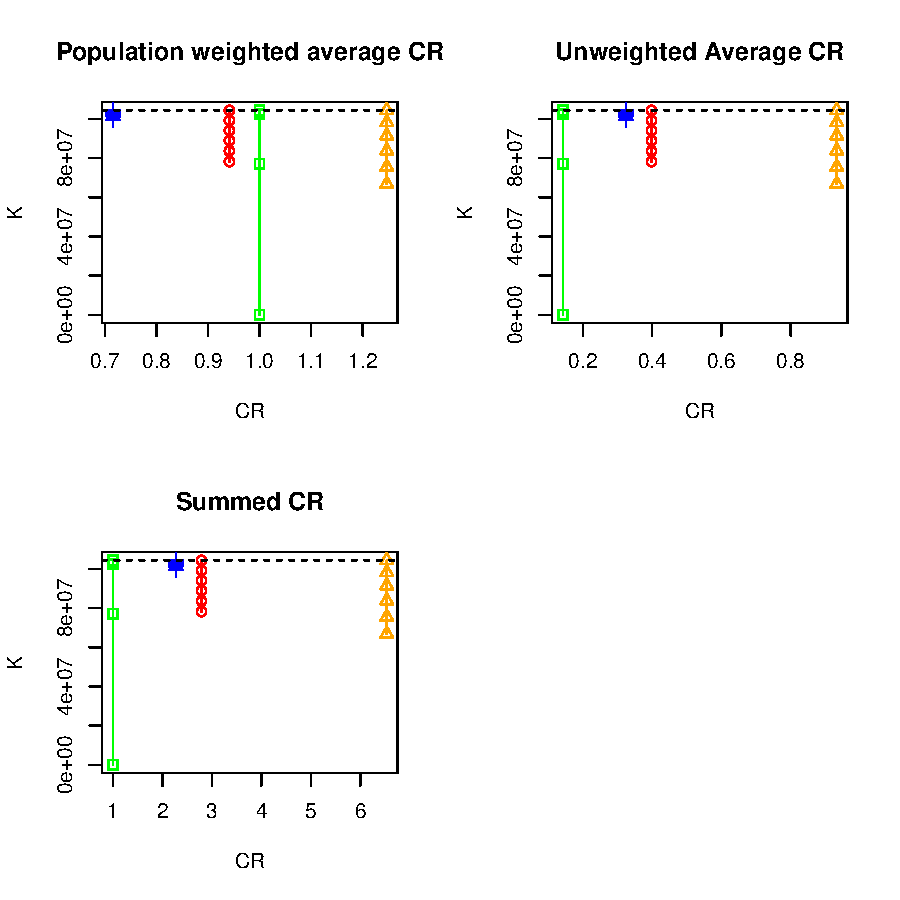
\includegraphics[width=\textwidth, height=.8\textwidth]{RGraphics-monarch_barcr_averageCR}
\caption{Perturbation results: Range of K values after perturbations to each node, X-axis represents {\bf{baseline population weighted $C^r$ values}} for each node}\label{fig:monarch_barcr_averageCR}
\end{center}
\end{figure}

\vspace{-.5cm}
\begin{tabular}{|c|c|c|}
\hline
{\color{green}Winter} & $\Box$ & non-breeding \\
\hline
{\color{red}South} & $\bigcirc$ & breeding \\
\hline
{\color{orange}Central} & $\triangle$ & breeding \\
\hline
{\color{blue}North} & $\diamond$ & breeding \\
\hline
\end{tabular}







\newpage
%########################################################%
\section{Population Distribution \texorpdfstring{$W^r$}{WR} - split seasons}

$W^r$ is calculated as the percent of the total population residing at a node. This calculation results in $W^r$ values for each node during each seaons. To get a consistent value for the network, we average (not weighted) across the seasons. The final numbers should sum to one.


\vspace{-.5cm}
\begin{figure}[H]
\begin{center}
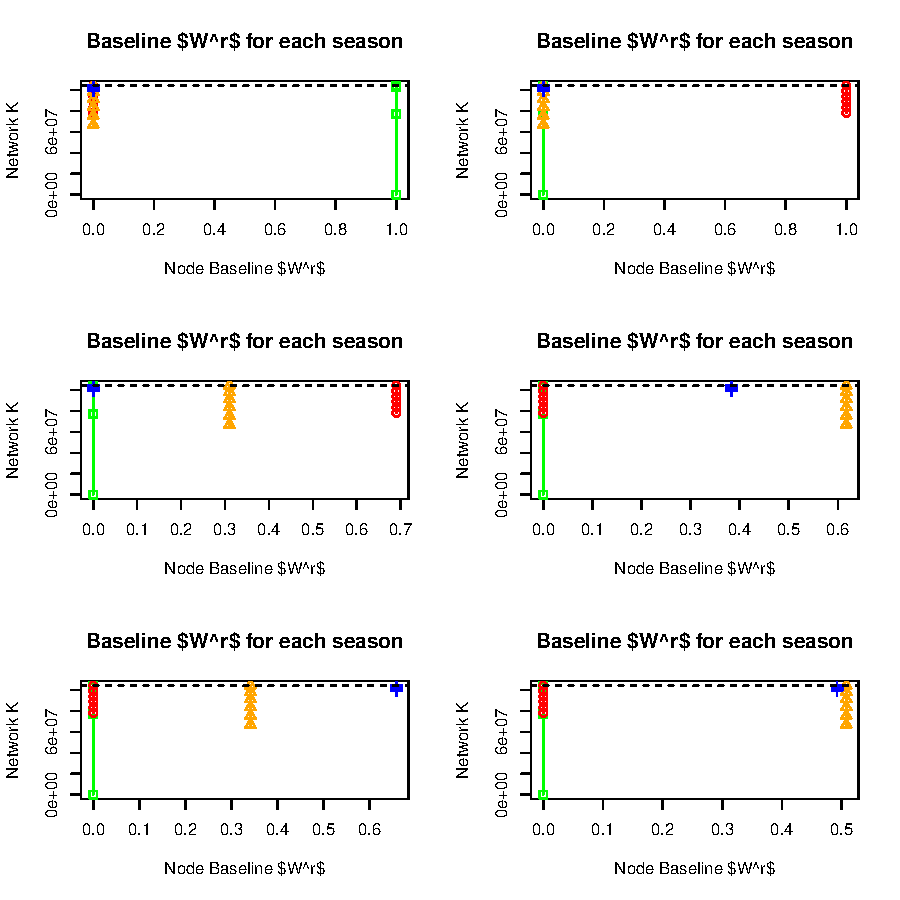
\includegraphics[width=.8\textwidth, height=.8\textwidth]{RGraphics-monarch_barcr_WR}
\caption{Perturbation results: Range of K values after perturbations to each node, X-axis represents baseline average $W^r$ value for each node}\label{fig:monarch_barcr_WR}
\end{center}
\end{figure}

\vspace{-.5cm}
\begin{tabular}{|c|c|c|}
\hline
{\color{green}Winter} & $\Box$ & non-breeding \\
\hline
{\color{red}South} & $\bigcirc$ & breeding \\
\hline
{\color{orange}Central} & $\triangle$ & breeding \\
\hline
{\color{blue}North} & $\diamond$ & breeding \\
\hline
\end{tabular}

%########################################################%
\section{CR - split seasons}

How does CR look if we split apart the seasons?


\vspace{-.5cm}
\begin{figure}[H]
\begin{center}
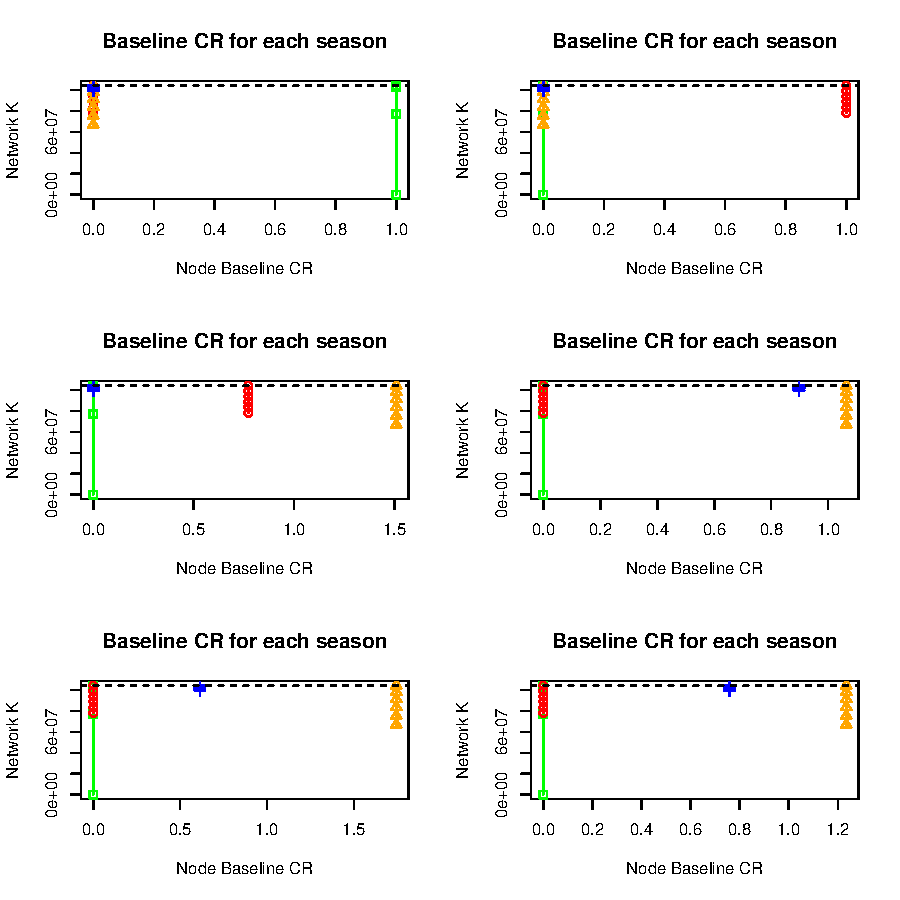
\includegraphics[width=.8\textwidth, height=.8\textwidth]{RGraphics-monarch_barcr_CRseasons}
\caption{Perturbation results: Range of K values after perturbations to each node, X-axis represents baseline average CR value for each node, here we have split up the seasons - no average}\label{fig:monarch_barcr_WR}
\end{center}
\end{figure}

\vspace{-.5cm}
\begin{tabular}{|c|c|c|}
\hline
{\color{green}Winter} & $\Box$ & non-breeding \\
\hline
{\color{red}South} & $\bigcirc$ & breeding \\
\hline
{\color{orange}Central} & $\triangle$ & breeding \\
\hline
{\color{blue}North} & $\diamond$ & breeding \\
\hline
\end{tabular}


\end{document}
